\chapter{Mapeamento de objetos para o Modelo Relacional}\label{cap:cap1}

\begin{flushright}
	\textit{
		Um ladrão rouba um tesouro, mas não furta a inteligência. \\
		Uma crise destrói um herança, mas não uma profissão. \\ Não importa se você não tem dinheiro, você é uma pessoa rica, \\ pois possui o maior de todos os capitais: a sua inteligência. \\ Invista nela. \textbf{Estude}!.
	} \\
	
	\textbf{Augusto Cury}
\end{flushright}

A tecnologia de orientação a objetos é consolidada como a forma mais usual para o desenvolvimento de softwares. Já, quando pensamos em banco de dados, os bancos relacionais forma os que tiveram maior exito e, sem dúvida, os Sistemas Gerenciadores de Banco de dados Relacionais (SGBDR) dominam o mercado. 

No entanto, essas duas tecnologias surgiram por meio de princípios teóricos muito diferentes. Segundo \citeonline{bezerra2016principios} o descasamento de informações \textit{(impedance mismatch)} é um termo utilizado para denotar o problema das diferenças entre as representações do modelo de objetos e do modelo relacional.

"Os princípios básicos do paradigma da orientação a objetos e do modelo relacional são bastante diferentes. No modelo de objetos, os elementos (objetos) correspondem a abstrações de comportamento. No modelo relacional, os elementos correspondem a dados no formato tabular \cite{bezerra2016principios}". Assim, neste capítulo, vamos apresentamos alguns detalhes a respeito dos diversos aspectos relativos ao mapeamento de objetos para um mecanismo de armazenamento persistente.

\section{Projeto de banco de dados}

Uma das principais atividades do projeto é o desenvolvimento do banco de dados. Essa atividade, durante o processo, normalmente é chamada de projeto de banco de dados. Tal projeto envolve diversas atividades, tais como:

\begin{itemize}
	\item Construção do esquema do banco de dados.
	\item Criação de índices2 para agilizar o acesso aos dados armazenados.
	\item Definição das estruturas de dados a serem utilizadas no armazenamento físico dos dados.
	\item Definição de visões sobre as dados armazenados.
	\item Atribuição de direitos de acesso (que usuários podem acessar que recursos).
	\item Definição de políticas de backup dos dados.
\end{itemize}

\subsection{Conceitos básicos do modelo de dados relacionais}

O modelo relacional, segundo \citeonline{bezerra2016principios}, se fundamenta no conceito de relação. De forma bastante simplista, pode-se pensar em uma relação como uma tabela, composta de linhas e de colunas. Cada relação possui um nome. Cada coluna de uma relação possui um nome e um domínio.

\begin{figure}[H]
	\centering
	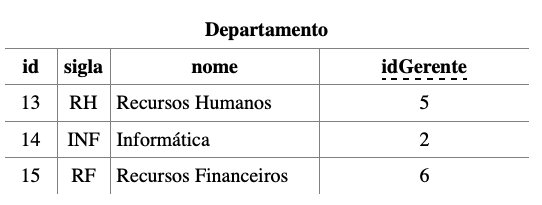
\includegraphics[scale=0.6]{imagens/banco1.png}
	\caption{Exemplo de relações em um banco de dados}
	\legend{Fonte: \cite{bezerra2016principios}}
	\label{fig:figura-01-banco-01}
\end{figure}

\subsubsection{Chave Primária}
Um conceito importante no modelo relacional é o de \textbf{chave primária}. Uma chave primária é uma coluna ou conjunto de colunas cujos valores podem ser utilizados para identificar unicamente cada linha de uma relação \cite{bezerra2016principios}. Note que a Figura \ref{fig:figura-01-banco-01} possue uma coluna chamada id. Essa coluna é a chave primária ds relação na qual aparece.

\subsubsection{Chave Estrangéira}\label{subsub:chave-estrangeira}
Outro conceito importante do modelo relacional é o de \textbf{chave estrangeira}. Linhas de uma relação podem estar associadas às de outras relações. Estas associações são representadas pela única maneira possível, considerando-se os recursos de notação do modelo relacional: deve existir, em uma das duas relações, uma coluna cujos valores fazem referência aos de uma coluna da outra relação. Na terminologia do modelo relacional, esta coluna de referência é denominada chave estrangeira. Em nossa Figura \ref{fig:figura-01-banco-01} a chave estrangeira é representada pelo campo idGerente, o qual apresenta-se tracejado.

\section{Mapeamento de objetos para o modelo relacional} 

Quando utilizamos um SGBD para gerenciar nossa base de dados e nosso armazenamento persistente de informações para um sistema de software orientado a objetos, há a necessidade de se realizar o mapeamento dos valores de atributos de objetos persistentes do sistema para tabelas. 

Assim, em nossa próxima sessão vamos aprender o procedimento de mapeamento de diversos elementos do modelo de classes para o modelo relacional. 

\subsection{Classe e seus atributos}

Segundo \citeonline{bezerra2016principios}, classes são mapeadas para relações. O caso mais simples é o de mapear cada classe como uma relação e cada um de seus atributos como uma coluna da relação correspondente. No entanto, muito frequentemente não há uma correspondência unívoca entre classes e relações. Pode ser que várias classes sejam mapeadas para uma única relação ou que uma classe seja mapeada para várias relações.

Para atributos o que vale de forma geral é que um atributo será mapeado para uma ou mais colunas. Lembre-se, também, de que nem todos os atributos são persistentes. Por exemplo, pode ser que uma classe Pedido tenha um atributo derivado, total, utilizado para guardar o valor total a ser pago por um pedido, mas que este atributo não seja armazenado no banco de dados.

\begin{figure}[H]
	\centering
	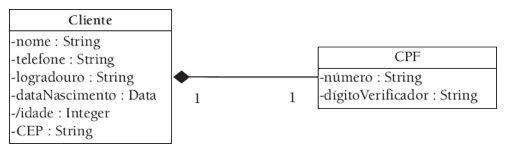
\includegraphics[scale=0.6]{imagens/mapeamento01.png}
	\caption{Classe cliente é CPF}
	\legend{Fonte: \cite{bezerra2016principios}}
	\label{fig:figura-01-banco-02}
\end{figure}

Considere a classe apresentada na Figura \ref{fig:figura-01-banco-02}. A Figura \ref{fig:figura-01-banco-03} exibe duas alternativas de mapeamento possíveis para essa classe. Note que, em ambos os casos, o atributo derivado idade não é mapeado. Além disso, nas duas alternativas, as classes \textbf{Cliente} e \textbf{CPF} são mapeadas para uma única relação. No entanto, na primeira alternativa, o CEP de um cliente é mapeado para uma relação separada e o atributo CEP da classe é dividido em duas partes (número e dígitoVerificador).

\begin{figure}[H]
	\centering
	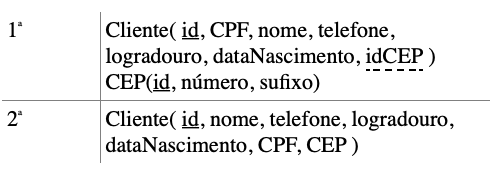
\includegraphics[scale=0.6]{imagens/mapeamento02.png}
	\caption{Classe cliente é CPF}
	\legend{Fonte: \cite{bezerra2016principios}}
	\label{fig:figura-01-banco-03}
\end{figure}

\section{Exercício de fixação}

Utilizando os conceitos até o momento apresentados, realize o mapeamento do digrama abaixo.

\begin{figure}[H]
	\centering
	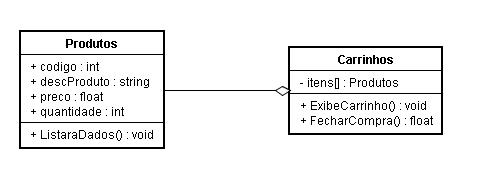
\includegraphics[scale=0.8]{imagens/agregacao22.jpg}
% 	\caption{Classe cliente é CPF}
% 	\legend{Fonte: \cite{bezerra2016principios}}
% 	\label{fig:figura-01-banco-03}
\end{figure}

\subsection{Associações}

Para que possamos mapear associações, nós utilizarmos o conceito de \textbf{chave estrangeira}. Uma chave estrangeira, como descrito na sub-sessão \ref{subsub:chave-estrangeira}, são utilizadas para relacionar linhas de relações diferentes ou linhas de uma mesma relação. Para isso, há três casos para mapeamento de associações, cada um correspondente a um tipo de conectividade.

\begin{figure}[H]
	\centering
	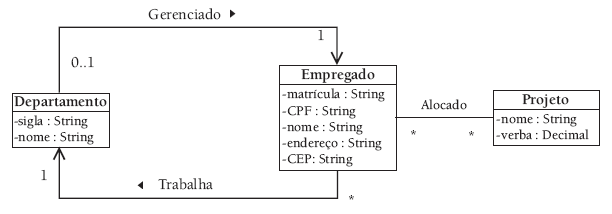
\includegraphics[scale=0.8]{imagens/tipos-de-conectividade.png}
	\caption{Diagrama de classes ilustrando os três tipos de conectividade em associações}
	\legend{Fonte: \cite{bezerra2016principios}}
	\label{fig:figura-01-banco-04}
\end{figure}

\subsubsection{Associação um-para-um}

Quando há uma associação um-para-um entre \textbf{Ca} e \textbf{Cb}, deve-se adicionar uma chave estrangeira em uma das duas relações para referenciar a chave primária da outra relação.

\textbf{Departamento(id, sigla, nome, idEmpregadoGerente)}

\textbf{Empregado( id, matrícula, CPF, nome, endereço, CEP )}

Contudo, há casos que a associação um-para-um pode ser mapeada para uma única relação, como no caso do diagrama apresentado na Figura \ref{fig:figura-01-banco-02}

\subsubsection{Associação um-para-muitos}

Em uma associação um-para-muitos entre objetos de \textbf{Ca} e de \textbf{Cb}, seja \textbf{Ca} a classe na qual cada objeto se associa com muitos objetos da classe \textbf{Cb}. Neste caso, deve-se adicionar uma chave estrangeira em \textbf{Ca} para referenciar a chave primária de \textbf{Cb} \cite{bezerra2016principios}.

Como exemplo, considere novamente a Figura \ref{fig:figura-01-banco-04}, na qual se apresenta a associação um para muitos Trabalha. A seguir é apresentada uma extensão do mapeamento anterior considerando essa associação.

\textbf{Departamento(id, sigla, nome, idEmpregadoGerente)}

\textbf{Empregado(id, matrícula, CPF, nome, endereço, CEP, idDepartamento)}

\subsubsection{Associações de conectividade muitos para muitos}

Quando há uma associação de conectividade muitos para muitos entre objetos de Ca e de Cb, uma relação de associação deve ser criada. Uma relação de associação tem o objetivo de representar a associação muitos para muitos entre duas ou mais relações \cite{bezerra2016principios}.

\textbf{Departamento(id, sigla, nome, idEmpregadoGerente)}

\textbf{Empregado(id, matrícula, CPF, nome, endereço, CEP, idDepartamento)}

\textbf{Alocação(id, idProjeto, idEmpregado, nome, verba)}

\textbf{Projeto(id, nome, verba)}

Assim, de forma geral, independente da conectividade, o conceito de chave estrangeira é sempre utilizado quando realizamos o mapeamento. Esta técnica é a mesma utilizada para a \textbf{agregação} ou para a \textbf{composição}. Contudo, para que se possa alcançar o comportamento esperado, devemos utilizar técnicas que envolvem os gatilhos (\textbf{triggers}) e procedimentos armazenados (\textbf{stored procedures}), os quais não serão tratados neste capítulo. 

\subsubsection{Associação reflexiva}

Uma associação reflexiva, ou também conhecida como auto-associação, é um tipo especial de associação. Contudo, o mapeamento aplicado a associações é igualmente ao aplicado em outras associações.

\begin{figure}[H]
	\centering
	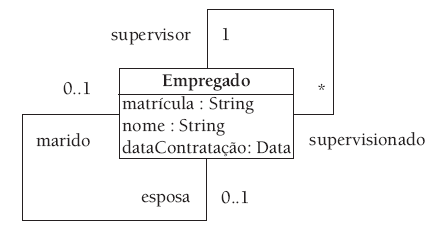
\includegraphics[scale=0.7]{imagens/reflexiva.png}
	\caption{Associações reflexivas entre objetos da classe Empregado}
	\legend{Fonte: \cite{bezerra2016principios}}
	\label{fig:figura-01-banco-05}
\end{figure}

Um possível mapeamento desse diagrama é apresentado a seguir. Note que as chaves estrangeiras idCônjunge e idSupervisor foram definidas na relação Empregado como era esperado, visto que ambas as associações são reflexivas.

\textbf{Empregado(id, matrícula, nome, dataContratação, idCônjunge, idSupervisor)}

\subsubsection{Associação ternária}

Associações ternárias, ou também conhecidas como associações n-árias, podem ser mapeadas por meio de um procedimento semelhante ao utilizado para associações binárias de conectividade muitos para muitos. Uma relação para representar a associação é criada e são adicionadas nelas chaves estrangeiras para as \textbf{n} classes participantes da associação. Se a associação ternária possuir uma classe associativa, os atributos dela são mapeados como colunas da relação de associação \cite{bezerra2016principios}.

\begin{figure}[H]
	\centering
	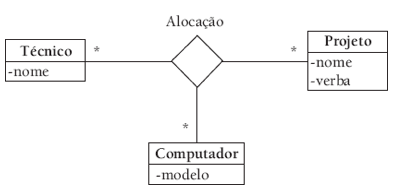
\includegraphics[scale=0.7]{imagens/terminaria.png}
	\caption{Associação terminária/N-ária}
	\legend{Fonte: \cite{bezerra2016principios}}
	\label{fig:figura-01-banco-06}
\end{figure}

\subsubitem{Generalização}

Há basicamente três alternativas de se mapear relacionamentos de generalização.

\begin{enumerate}
	\item Uma relação para cada classe da hierarquia;
	\item Uma relação para toda a hierarquia;
	\item Uma relação para cada classe concreta da hierarquia.
\end{enumerate}

Assim, vamos aplicar as três formas de mapeamento para o diagrama de classe abaixo.

\begin{figure}[H]
	\centering
	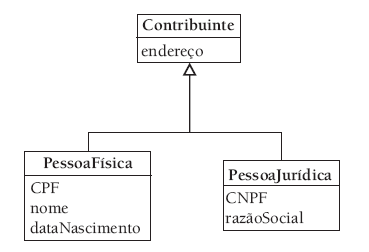
\includegraphics[scale=0.7]{imagens/generalizacao.png}
	\caption{Hierarquia de generalização}
	\legend{Fonte: \cite{bezerra2016principios}}
	\label{fig:figura-01-banco-07}
\end{figure}

Realizando o mapeamento por meio das três alternativas possíveis, obtemos o seguinte resultado:
\\

Alternativa 1

\textbf{Contribuinte(id, endereço)}

\textbf{PessoaFísica(id, nome, dataNascimento, CPF, idContribuinte)}

\textbf{PessoaJurídica(id, CNPJ, razãoSocial, idContribuinte)}
\\

Alternativa 2

\textbf{Pessoa(id, nome, endereço, dataNascimento, CPF, CNPJ, razãoSocial, tipo)
}
\\

Alternativa 3

\textbf{PessoaFísica(id, dataNascimento, nome, endereço, CPF)}

\textbf{PessoaJurídica(id, CNPJ, endereço, razãoSocial)}


\section{Exercício de fixação}

Utilizando os conceitos até o momento apresentados, realize o mapeamento dos diagramas abaixo.

1. 
\begin{figure}[H]
	\centering
	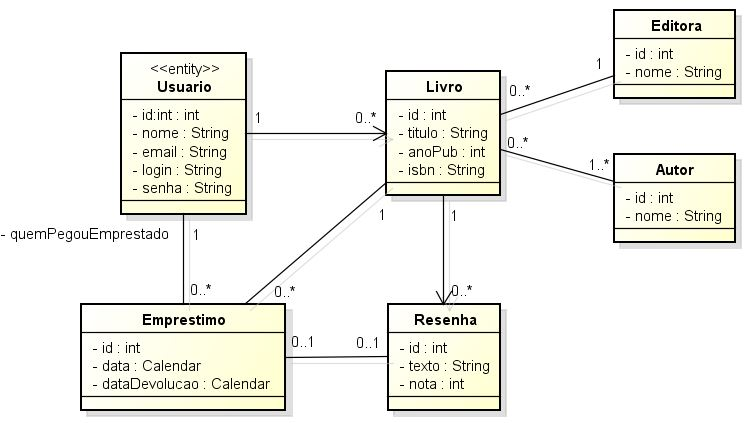
\includegraphics[scale=0.7]{imagens/dominio1.jpg}
\end{figure}

\begin{figure}[H]
	\centering
	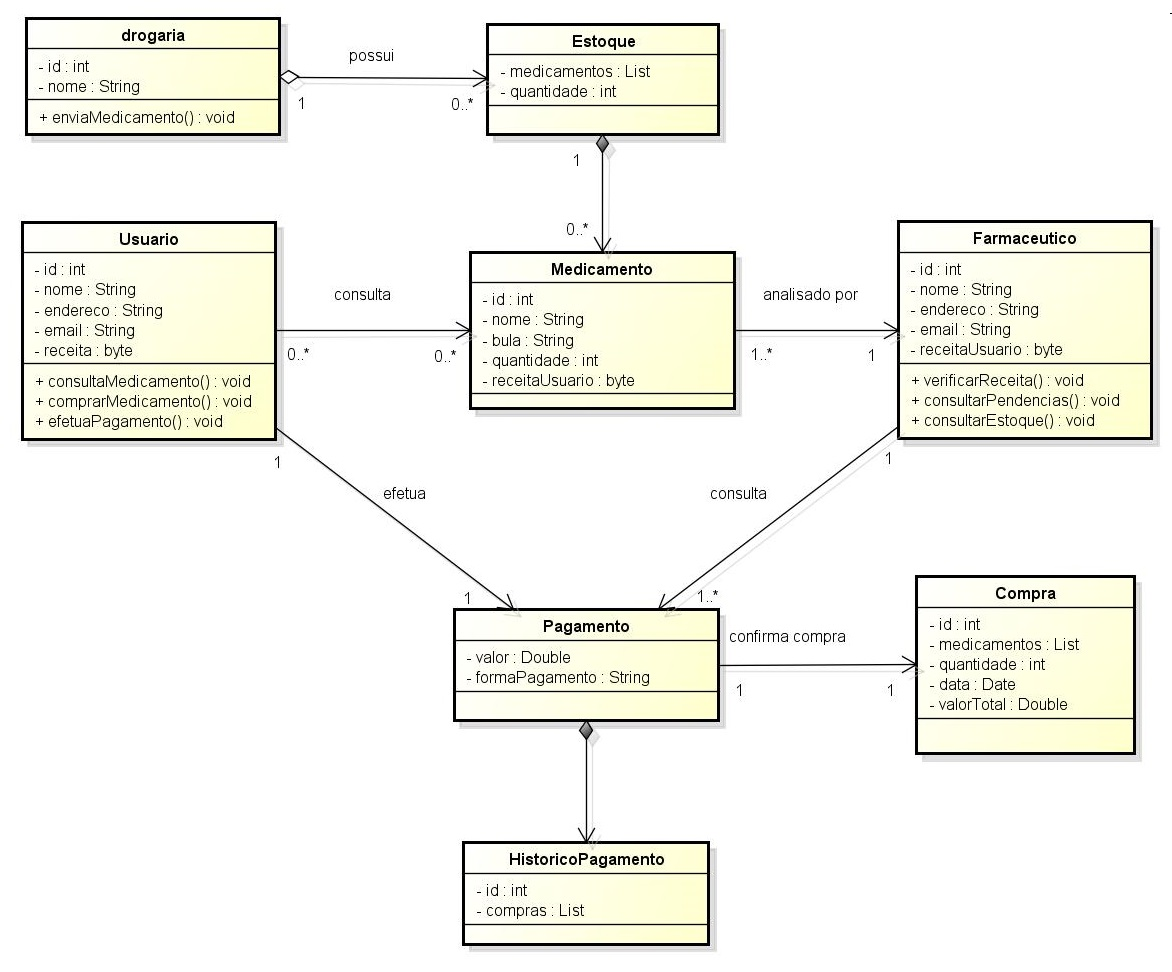
\includegraphics[scale=0.5]{imagens/farmacia_classdiagram.jpg}
\end{figure}

\begin{figure}[H]
	\centering
	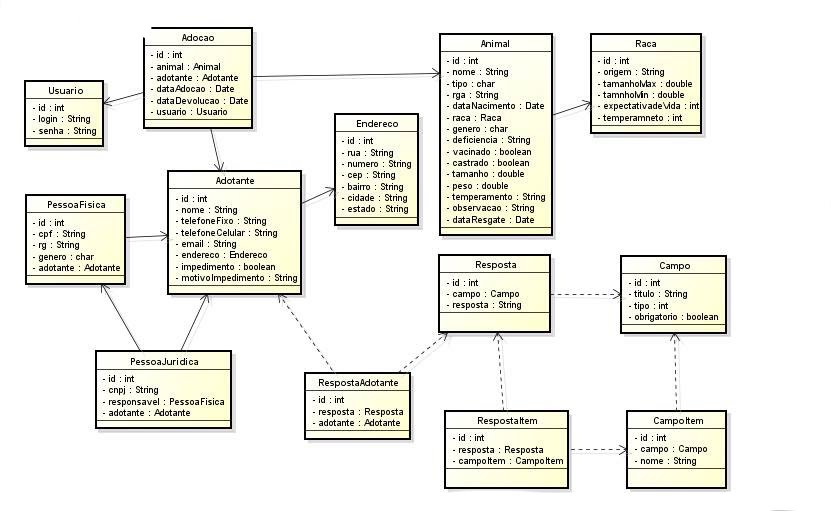
\includegraphics[scale=0.6]{imagens/diagrama-de-classe-2.jpg}
\end{figure}